\documentclass[a4paper,12pt]{article}

%Class
	%\documentclass[a4paper,12pt]{article}

%Packages
	\usepackage{amsmath}					% Standard maths
	\usepackage{amssymb}					% Standard maths
	\usepackage{amsthm}						% Standard maths
	\usepackage{thmtools, thm-restate}% Theorem styles
	\usepackage{mathtools}
	\usepackage[newzealand]{babel}% Date/time in British format (yes, I know it says NZ)
	\usepackage{datetime}					% Date/time
	\usepackage{multirow}					% For stacked subscripts
	\usepackage{xcolor}						% For colour!
	\usepackage[normalem]{ulem}		% For strikeout
	\usepackage{isomath}
	\usepackage{fancyhdr}					% For the headers
	\usepackage{mfirstuc}					% For the headers
	\usepackage[hmargin=1in,top=0.8in,bottom=1in]{geometry} % Page margins more reasonable
	\usepackage{graphicx}					% For including graphics
	%\usepackage{float}						% For something
	\usepackage{enumitem}					% For numbering tweaks
	\usepackage[margin=15pt,font={small},labelfont=bf,format=hang]{caption} % Changing caption style
	\usepackage{url}
	\usepackage[hidelinks]{hyperref}	% For hyperlinks
	\usepackage{breakurl}
	\usepackage{cleveref}
	\usepackage[scaled=.92]{helvet}
	\usepackage[]{FiraSans}
	\usepackage[T1]{fontenc}
	\usepackage{comment}
	\newbool{show_question}
	\newbool{show_solution}
	\newbool{show_commentary}
	\newcommand{\solutioninheading}{\ifbool{show_solution}{: SOLUTIONS\ifbool{show_commentary}{ \& FEEDBACK}{}}{}}
	
	\usepackage{pgfplots}
\newcommand{\ep}{\varepsilon}	

    \newcommand{\question}[3]{
    	\item %\textbf{#1} \par \medskip % Title
    	%
    	\ifbool{show_question}{#2}{} % Question
    	%
    	%
    	\ifbool{show_question}{\ifbool{show_solution}{\par\medskip\textbf{Solution:}}{}}{} % Both
    	\ifbool{show_solution}{#3}{} % Answer
    }

\usepackage[most]{tcolorbox}

%MATHEMATICAL SHORTCUTS
%Two and three-part definitions
	\newcommand{\twopartdef}[4]
	{	\left\{
			\begin{array}{ll}
				#1 & \mbox{if } #2 \\
				#3 & \mbox{if } #4
			\end{array}
		\right.}
%	\newcommand{\threepartdef}[6]
%	{	\left\{
%			\begin{array}{ll}
%				#1 & \mbox{if } #2 \\
%				#3 & \mbox{if } #4 \\
%				#5 & \mbox{if } #6
%			\end{array}
%		\right.}
%Blackboard bold	
	\newcommand{\N}{{\mathbb N}} 
	\newcommand{\R}{{\mathbb R}} 
	\newcommand{\C}{{\mathbb C}} 
	%Curly letters
%	\newcommand{\E}{{\mathcal E}}	
%	\newcommand{\F}{{\mathcal F}} 
%	\newcommand{\Null}{{\mathcal N}} 
%	\newcommand{\R}{\mathcal{R}} 
%	\newcommand{\Z}{\mathcal{Z}} 
%Uprights
	\newcommand{\D}{{\mathrm D}}
	\renewcommand{\d}{{\mathrm d}}
%Easy Greeks
%	\def\a{\alpha}
%	\def\g{\gamma}
%	\newcommand{\e}{{\varepsilon}}
%	\newcommand{\la}{{\lambda}}  
%	\newcommand{\om}{{\Omega}}
	\renewcommand{\epsilon}{\varepsilon}
	
%Vector operators
	\def \p {\partial}
	\newcommand{\del}{{\nabla}}
	\newcommand{\grad}{{\nabla}}
	\newcommand{\cross}{{\times}}
	\newcommand{\Lap}{{\nabla^2}} 
	\newcommand{\vnabla}{\boldsymbol{\nabla}}
%Arrows
%	\newcommand{\goesto}[1]{\xrightarrow[#1]{}}
%hats
%	\newcommand{\nhat}{\widehat{\v{n}}}
%	\newcommand{\shat}{\widehat{\v{s}}}
	\renewcommand{\hat}{\widehat}
%Note to self
%	\newcommand{\note}[1]{[\textbf{\textsl{\MakeUppercase{#1}}}]}
	
%Stress tensor
%	\newcommand{\T}{\vg{\sigma}}

% Vectors, quaternions etc.
\renewcommand{\v}[1]{\mathbfit{#1}}      % Generic vector
\newcommand{\vc}[1]{\bm{\mathcal{#1}}}      % vector mathcal
\newcommand{\uv}[1]{\widehat{\mathbfit{#1}}}      % Generic unit vector
\newcommand{\q}[1]{\mathsfbfit{#1}}        % Generic quaternion
\renewcommand{\t}[1]{\mathsfbfit{#1}}	 % Generic tensor
\newcommand{\m}[1]{\mathsfbfit{#1}}	 % Generic matrix
\newcommand{\vu}[1]{\mathbf{#1}}         % Upright vector (for zero vector)
\newcommand{\qu}[1]{\mathbf{#1}}       % Upright quaternion (for zero quaternion)
\newcommand{\tu}[1]{\bm{\mathsf{#1}}}	 % Upright tensor (for zero tensor)

%Real and imaginary
\renewcommand{\Re}{\operatorname{Re}}
\renewcommand{\Im}{\operatorname{Im}}
	
%Non-dim numbers
%	\renewcommand{\Re}{\operatorname{Re}}
%	\newcommand{\Bi}{\operatorname{Bi}}
%	\newcommand{\Fo}{\operatorname{Fo}}
	
%Misc
\DeclareMathSymbol{\Delta}{\mathalpha}{operators}{1} % Keeps Delta upright
\DeclareMathSymbol{\Gamma}{\mathalpha}{operators}{0} % Keeps Gamma upright
	\newcommand{\cosec}{\operatorname{cosec}}
	\newcommand{\cosech}{\operatorname{cosech}}
	\newcommand{\sech}{\operatorname{sech}}
	\newcommand{\tr}{\operatorname{tr}}
	\newcommand{\erf}{\operatorname{erf}}
	\newcommand{\order}{\mathcal{O}}
%	\newcommand{\V}{\mathcal{V}} % 	CurlyV = (Bi V) / (1 + Bi)

% Differentiating 
\newcommand{\fd}[2]{\mathchoice{\frac{\d #1}{\d #2}}{\d #1/\d #2}{\d #1/\d #2}{\d #1/\d #2}}
\newcommand{\fdd}[2]{\mathchoice{\frac{\d^2 #1}{\d #2^2}}{\d^2 #1/\d #2^2}{\d^2 #1/\d #2^2}{\d^2 #1/\d #2^2}}
\newcommand{\fddd}[2]{\mathchoice{\frac{\d^3 #1}{\d #2^3}}{\d^3 #1/\d #2^3}{\d^3 #1/\d #2^3}{\d^3 #1/\d #2^3}}
\newcommand{\fdddd}[2]{\mathchoice{\frac{\d^4 #1}{\d #2^4}}{\d^4 #1/\d #2^4}{\d^4 #1/\d #2^4}{\d^4 #1/\d #2^4}}
\newcommand{\fdn}[3]{\mathchoice{\frac{\d^{#1} #2}{\d #3^{#1}}}{\d^{#1} #2/\d #3^{#1}}{\d^{#1} #2/\d #3^{#1}}{\d^{#1} #2/\d #3^{#1}}}
\newcommand{\pd}[2]{\mathchoice{\frac{\p #1}{\p #2}}{\p #1/\p #2}{\p #1/\p #2}{\p #1/\p #2}}
\newcommand{\pdd}[2]{\mathchoice{\frac{\p^2 #1}{\p #2^2}}{\p^2 #1/\p #2^2}{\p^2 #1/\p #2^2}{\p^2 #1/\p #2^2}}
\newcommand{\pddmixed}[3]{\frac{\p^2 #1}{\p #2 \p #3}}
\newcommand{\pddd}[2]{\frac{\p^3 #1}{\p #2^3}}
\newcommand{\pdn}[3]{\mathchoice{\frac{\p^{#1} #2}{\p #3^{#1}}}{\p^{#1} #2/\p #3^{#1}}{\p^{#1} #2/\p #3^{#1}}{\p^{#1} #2/\p #3^{#1}}}
	
	% Misc
\newcommand{\e}{\mathrm{e}}
\renewcommand{\i}{\mathrm{i}}
\newcommand{\dx}{\,\mathrm{d}x}
\newcommand{\dy}{\,\mathrm{d}y}
\renewcommand{\epsilon}{\varepsilon}
\renewcommand{\Re}{\operatorname{Re}}
\newcommand{\Four}{\mathcal{F}}
	\definecolor{nem-red}{HTML}{FFEDF0}
\definecolor{nem-dark-red}{HTML}{d21f3c}
	\newenvironment{nem}{\begin{tcolorbox}[colback=nem-red,colframe=nem-dark-red,breakable,enhanced,parbox=false,title={\sf\small{Non-examinable}}]}{\end{tcolorbox}}
	
\newenvironment{colour-box-breakable}[3]{
\setlist[itemize]{topsep=-\parskip,before=\vspace{-2mm},itemsep=3pt}
%\setlength{\parskip}{0pt}
\begin{tcolorbox}[
	enhanced,
    breakable,
	colback=#2,
	colframe=#1,
	colbacktitle=#2, 
	frame hidden,
    boxrule=0pt,
    leftrule=2pt,
	toptitle=2.5mm,
	bottomtitle=-.5mm, 
    pad before break=1pt,
	pad after break=6pt,
	parbox=false,
	bottom=10pt,
	%grow to right by=0.5mm,
    %grow to left by=-0.2mm,
	sharp corners=west,
  	fonttitle={\sf\small},
	fontupper={\small},
	title={\color{#1}#3}, 
  	overlay first={
	  \fill[#1]
      ([xshift=2pt]frame.north west) --
      ([xshift=2pt]frame.south west) --
      ([xshift=0pt]frame.south west) --
      ([yshift=-2pt]frame.north west) arc
      [radius=2pt,start angle=180,end angle=90]--
      cycle;
    },
     overlay unbroken={
	  \fill[#1]
      ([xshift=2pt]frame.north west) --
      ([xshift=2pt]frame.south west) arc
      [radius=2pt,start angle=-90,end angle=-180] --
      ([yshift=-2pt]frame.north west) arc
      [radius=2pt,start angle=180,end angle=90]--
      cycle;
    },
  	overlay last={
	  \fill[#1]
      ([xshift=2pt]frame.north west) --
      ([xshift=2pt]frame.south west) arc
      [radius=2pt,start angle=-90,end angle=-180] --
      ([yshift=-2pt]frame.north west) --
      ([yshift=0pt]frame.north west) --
      cycle;
    },
]}{\end{tcolorbox}}

\definecolor{commentary-green}{HTML}{FBF3EE}
\definecolor{commentary-dark-green}{HTML}{c57a44}

\newcommand{\commentary}[1]
{
\ifbool{show_commentary}{
	\begin{colour-box-breakable}
		{commentary-dark-green}
		{commentary-green}
		{\footnotesize\raisebox{-2pt}{
\includegraphics[width=1em]{../common/squirrel.png}}\,\,Feedback}
	#1
\end{colour-box-breakable}
	}{}
}
%}{
%  \newenvironment{commentary}{\commentaryA}{\endcommentary}
%}

%Depth of display breaks to allow	
	\allowdisplaybreaks[1]

%How deep do we want the Table of Contents to go?	
%	\setcounter{tocdepth}{1}

%Sections
\makeatletter
\renewcommand{\section}{\@startsection
{section}%                   % the name
{1}%                         % the level
{0mm}%                       % the indent
{-\baselineskip}%            % the before skip
{0.5\baselineskip}%          % the after skip
{\normalfont\bfseries}} % the style
\makeatother

% Wavy underline
\makeatletter
\font\sixly=lasyb10 scaled 1200
\def\tinners{\bgroup \markoverwith{\lower8.5\p@\hbox{\sixly \char58}}\ULon}
\makeatother
\newcommand{\answer}[1]{\tinners{\; #1 \;}}

%Setting the footnotes to use *,**,+ etc rather than 1,2,3	
\renewcommand{\thefootnote}{\fnsymbol{footnote}}

%Italic quote environment
%\newenvironment{quoteitalic}{\begin{quote}\itshape}{\end{quote}}

%Heading
\newcommand{\heading}[2]{
\setlength{\parindent}{0pt}
\textbf{MATH3171 (Mathematical Biology III)}

\textbf{YEAR 2025--26, \MakeUppercase{#1} TERM}
\setlength{\parskip}{3ex}

\textbf{\MakeUppercase{#2}}
%
\setlength{\parskip}{2ex}

}

%========================================================================================================================
%DOCUMENT BEGINS HERE!


\begin{document} 
\newcommand{\sol}[1]{\\ \hrule\hfill \\ \textcolor{blue}{\textbf{SOLUTION:}} #1 \\ \hrule\hfill}\heading{Epiphany}{Problem sheet 6: Solutions}\setbool{show_commentary}{true}
%\newcommand{\sol}[1]{}\heading{Epiphany}{Problem sheet 6} \setbool{show_commentary}{false}
\renewcommand*{\thefootnote}{\arabic{footnote}}

%

%
  This problem sheet is due in by \textbf{5pm} on \textbf{Wednesday 18 February 2026}. You may submit it on paper to my office (\textsc{mcs}\,3114) or electronically on Gradescope.

\textbf{Topics covered}: Chapter 10
\begin{enumerate}
\item \textbf{Allee population dynamics with spatial variations}
\begin{enumerate}
    \item Consider a population $u(t)$ evolving according to \begin{equation}\label{Allee_ODE}
         \fd{u}{t} =ru\left (\frac{u}{A}-1 \right ) \left(1-\frac{u}{K} \right),
         \end{equation}
    with the parameters $r>0$, $K>0$ and $0 < A < K$. Explain the biological interpretation of the three parameters. 
    \sol{
 Interpretation of the three parameters:
    \begin{itemize}
        \item $r$ is the growth rate of the population,
        \item $K$ the maximum carrying capacity,
        \item $A$ the Allee parameter determining the threshold population.
    \end{itemize}
    \hspace{1cm}
    }\commentary{Broadly this part was fine, and credit was given generously. It is worth noting that $r$ is really a timescale of the whole process, both growth and death of the population, but for this course simpler descriptions are fine.}    
    \item Using linear stability analysis and/or a graphical representation of the phase space, explain the behaviour of the population $u$ satisfying \cref{Allee_ODE} for different initial conditions. 
    \sol{
 This example is exactly done in the Michaelmas portion of the course. The three equilibria are $u_0=0, A, K$, which can be seen as the right-hand-side is factored in terms of these three roots. Stability can be determined by signing $f'(u_0)$ in each case, where we compute:
      $$
      f'(u_0)=r\left (\frac{u_0}{A}-1 \right ) \left(1-\frac{u_0}{K} \right) + \frac{ru_0}{A} \left(1-\frac{u_0}{K} \right) - \frac{ru_0}{K}\left (\frac{u_0}{A}-1 \right ).
      $$
This is a nice form as for each of our equilibria above, two of the terms drop out in each case. So we have:
      \begin{itemize}
          \item $f'(0)<0$ so $u_0=0$ is stable,
          \item $f'(A)>0$ so $u_0=A$ is unstable,
          \item $f'(K)<0$ so $u_0=K$ is stable.
      \end{itemize}
      
      Another method is to copmpute this graphically by plotting $f'(u)$ agbainst $u$:
      
      \begin{center}
          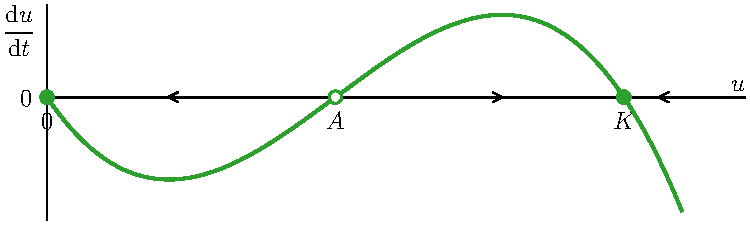
\includegraphics{allee-phase.pdf}
      \end{center}
      
      For the initial population $u(0)$,
      \begin{itemize}
          \item if $u(0)>A$ then $u \to K$ as $t \to \infty$,
          \item if $u(0)<A$ then $u \to 0$ as $t \to \infty$, so this models death of a sufficiently small population. 
      \end{itemize}
      \hspace{1cm}
    }\commentary{Very few issues for this question, but please do make sure you understand both the graphical and analytical approaches for stability, and what they tell you about how different initial data $u(0)$ evolve.}  
   \item Consider the spatial model for $u(x,t)$,
    \begin{equation}\label{Allee_PDE}
    \pd{u}{t} =D \nabla^2 u + ru\left (\frac{u}{A}-1 \right ) \left(1-\frac{u}{K} \right), \quad x \in \Omega = [0,L],\end{equation}  
     where $u$ satisfies Dirichlet conditions on its boundaries of the form $u = u_B$ for $x =0,L$, for some constant parameter value $u_B\geq0$. For what values of $u_B$ do spatially homogeneous equilibria exist? For all cases where they do exist, use a linear stability analysis to determine their stability as a function of the model parameters. For any of these cases where the spatial model can give a different stability prediction from the ODE, compute the critical domain length, $L_c$, where the stability of a spatially homogeneous equilibrium changes.
     \sol{
 Spatially homogeneous equilibria will exist only when $u_B=u_0$ for one of the three kinetic equilibria,
    \begin{equation*}
        u_B = 0, \quad u_B=A \quad\text{or}\quad u_B=K,    
    \end{equation*}
    and in each case there will only be a single equilibrium. 
    
    \paragraph{First consider $u_B=0$.} The only spatially homogeneous equilibrium in this case is $u_0=0$, as the other two would not satisfy the boundary conditions. Linearising about this equilibrium with $u=u_0+\varepsilon u_1$, we find: 
    $$
        \pd{u_1}{t} = D\pdd{u_1}{x} -ru_1, \quad u_1(0,t)=u_1(L,t)=0,
    $$
    and hence perturbation growth rates (determined by $U = \exp(\lambda_k t)\sin(k\pi x/L)$) are: 
    $$
    \lambda_k = -D\left(\frac{k \pi}{L}\right)^2 -r, \quad k=1,2,3,\dots
    $$
    and hence $\lambda_k < 0$ so this equilibrium is always stable. 
    
    \paragraph{Similarly we find for $u_B=A$:} 
    $$
    \lambda_k = -D\left(\frac{k \pi}{L}\right)^2 +r\left(1-\frac{A}{K}\right), \quad k=1,2,3,\dots
    $$
    which is more interesting. 
    
    As $A<K$, we have that $1-A/K>0$ so that this equilibrium is unconditionally unstable in the ODE case. But here, as $k=1$ is the smallest spatial eigenvalue, we can have $\lambda_1$ with a negative sign for sufficiently small values of $L$, as in the `harsh environment' case seen in the lecture notes. We find a critical domain length: 
    $$
    L_c = \pi \sqrt{\frac{DK}{r(K-A)}},
    $$
    such that $L>L_c$ makes $u_0=A$ unstable, but $L < L_c$ makes $u_0=A$ stable. 

    \paragraph{For $u_B=K$:} we find exactly the same result as in $u_B=0$, with the equilibrium always being stable as long as it exists. The calculation is essentially identical in this case, except with $f'(K) = r(1-K/A)$, which is negative as $K>A$ so $K/A>1$.
     }\commentary{A few issues/comments here:
     \begin{itemize}
         \item It is worth really understanding why there is only ever at most one equilibrium where $u_B = 0, A,$ or $K$. Any solution $u(t,x)$, which includes equilibrium solutions, \emph{must} satisfy the boundary conditions.
         \item You do not need to work out the separation of variables solution every time, or even the linearization, unless you are asked to do this precisely. As long as you know what the solution ansatz is, or what the linear equation is, you can just write it down.
         \item It is important to understand why $k=1$ gives the largest growth rate here, and why this can then impact stability.
     \end{itemize}}  
    \item Without redoing the linear stability analysis, explain what is different about the number and stability of equilibria of \cref{Allee_PDE} in the case of zero Neumann (no-flux) boundary conditions. 
    \sol{
    With zero Neumann conditions, we would allow any of the three homogeneous equilibria (as they all satisfy the boundary condition, since constants have zero derivative). The stability of the three equilibria would also not change from the ODE case, as $\lambda_0=f'(u_0)$. corresponding to $k=0$. is the largest growing mode, which is exactly what the ODE linear stability analysis gives as the growth rate.
    }\commentary{No major issues here except some people did not explain both points that the allowed equilibria are different here (i.e.~all three equilibria are permitted) and that the stability is the same as in the ODE case.}  
\end{enumerate}

\item \textbf{Separation of Variables}
    Consider the linear reaction-diffusion equation:
    \begin{equation}\label{sv_eqn}
        \pd{u}{t} = D\pdd{u}{x} + au, \quad x \in [0,L], \,\, t > 0,
    \end{equation}
    where $a$ is a constant, with the boundary conditions
    \begin{equation}
        \pd{u}{x}(0,t)=\pd{u}{x}(L,t)=0.
    \end{equation}
    \begin{enumerate}
        \item Assuming a solution of the form $u(x,t) = T(t)X(x)$, apply separation of variables to this equation and determine the equations solved by the functions $T$ and $X$. 
        \sol{
Making the substitution into \cref{sv_eqn} we have,
$$
T'(t)X(x) =  DT(t)X''(x) + aT(t)X(x).
$$
Dividing through by $T(t)X(x)$, and dropping the dependence on $x$ and $t$, we have
$$
\frac{T'}{T} = D\frac{X''}{X} + a = \lambda,
$$
where we have introduced a constant $\lambda$ as the left-hand side is a function of $t$ only, and the right-hand side a function of $x$ only. We therefore have the equations,
$$
T' = \lambda T, \quad X'' + \frac{a-\lambda}{D}X = 0.
$$
        }\commentary{Broadly this was done well, though it is helpful to ensure you understand where the constant comes from which motivates the entire idea of separable solutions.}  
        \item Solve for $T$ and $X$ explicitly. Use these solutions to write out the full solution for $u(x,t)$ given some initial condition $u(x,0)=f(x)$.
        \sol{
        The $T$ equation is easy to solve as $T = e^{\lambda t}$. The $X$ equation will depend on the sign of $(a-\lambda)/D$, as in the notes for the heat equation. The only permissible signs are when $(a-\lambda)/D\geq 0$, as otherwise the solutions will be exponentials that cannot satisfy the boundary conditions (see the solution of the heat equation in the notes if this is unfamiliar). So the solutions for $X$ are:
        $$
        X = A\cos\left(\sqrt{\frac{a-\lambda}{D}}x \right)+B\sin\left(\sqrt{\frac{a-\lambda}{D}}x \right).
        $$

        Applying the boundary conditions (that is, $X'(0)=X'(L)=0$), we have that $B=0$ and $$\sqrt{\frac{a-\lambda}{D}} = \frac{k\pi}{L}\implies \lambda=a-D\left(\frac{k\pi}{L}\right)^2.$$ 
        Importantly we note that $k=0$, when $\lambda = a$, is also a solution having a constant value.

        So the full solution can be written as,
        $$
         u(x,t) = \sum_{k=0}^\infty A_ke^{\displaystyle\left(a-D\frac{k\pi}{L}\right)^2 t}\cos\left( \frac{k\pi x}{L}\right),
        $$
        and we can use orthogonality of the cosine functions to compute the coefficients $A_k$ from the initial conditions as,
        $$
        A_k = \frac{\int_0^L \cos\left( \frac{k\pi x}{L}\right)f(x) dx}{\int_0^L\cos\left( \frac{k\pi x}{L}\right)^2 dx}, k=0,1,2,3,\dots
        $$
        }\commentary{A couple of issues happened occasionally:
        
        \begin{itemize}
            \item Some students were not careful about the sign of the constant term in the equation for $X(x)$ ($a-\lambda$ above). This is intimately related to what kinds of functions satisfy the boundary conditions, and is a key idea from Calculus and last year's methods course.
            \item There were a number of errors in solving for the initial conditions. While this is not something you will be examined on directly in this course, it is important to understand that the initial conditions do play a role in determining these solutions (and are connected to what we mean by a `perturbation' in linear stability analysis).
        \end{itemize}}  
        \item In deriving your solution above, the constant $a$ appeared in either the $X$ equation, or in the $T$ equation. Which of these choices makes the separation of variables arguments easier/more familiar? You may have to sketch out the argument in both cases to see this.
        \sol{
        If we had instead put the constant $a$ on the $T$ equation, and used a different constant $\rho$ instead of $\lambda$, we could have solved for $T = e^{(a+\rho)t}$, and our equation for $X$ would have been identical to the one for the heat equation, so we could have just written down the cosine functions above. The point here is to notice that we can separate the time and space parts of the equation, and that the linear term $au$ just shifts the growth rates, without changing the structure of the solution at all.
        }\commentary{Mostly this was just to get you to think, and to connect different ways of solving these problems. There isn't a `correct' answer as these different ways are all equivalent.}  
    \end{enumerate}
    

\end{enumerate}

    
\end{document}